\documentclass[10pt,twocolumn,letterpaper]{article}

\usepackage{cvpr}
\usepackage{times}
\usepackage{epsfig}
\usepackage{graphicx}
\usepackage{amsmath}
\usepackage{amssymb}

% Include other packages here, before hyperref.
\usepackage{glossaries}
\newacronym{dqn}{⟨DQN⟩}{⟨deep Q-network⟩}
% If you comment hyperref and then uncomment it, you should delete
% egpaper.aux before re-running latex.  (Or just hit 'q' on the first latex
% run, let it finish, and you should be clear).
\usepackage[pagebackref=true,breaklinks=true,letterpaper=true,colorlinks,bookmarks=false]{hyperref}

\cvprfinalcopy % *** Uncomment this line for the final submission

\def\cvprPaperID{****} % *** Enter the CVPR Paper ID here
\def\httilde{\mbox{\tt\raisebox{-.5ex}{\symbol{126}}}}

% Pages are numbered in submission mode, and unnumbered in camera-ready
\ifcvprfinal\pagestyle{empty}\fi
\begin{document}

%%%%%%%%% TITLE
\title{Reinforcement learning on playing Space Invaders and Breakout simultaneously}

\author{Strobel Maximilian\\
{\tt\small max.strobel@tum.de}
\and
Werhahn Maximilian\\
{\tt\small maxi.werhahn@gmx.de}
\and
Kiener Martin\\
{\tt\small martin.kiener@tum.de}
\and
Seferis Emmanouil \\
{\tt\small ga62cac@tum.de}
}


\maketitle
%\thispagestyle{empty}

%
% Proposal I
%
\section*{Project Proposal}

\section{Introduction}
We want to train an intelligent agent, who is capable of playing Space Invaders and Breakout simultaneously with the same inputs. During a first step we want to implement a \gls{dqn} with convolutional layers to get above the score of random play for either of the two games. In the next step we want to gain average human performance by optimizing hyperparameters. Afterwards we attempt to optimize the networks architecture to perform on an above human level. Finally we want to let the agent play both games at the same time with the restriction of only being able to send the same inputs to both games. This is why we chose Breakout and Space Invaders, since the valid inputs are almost the same.

\begin{figure}[!h]
  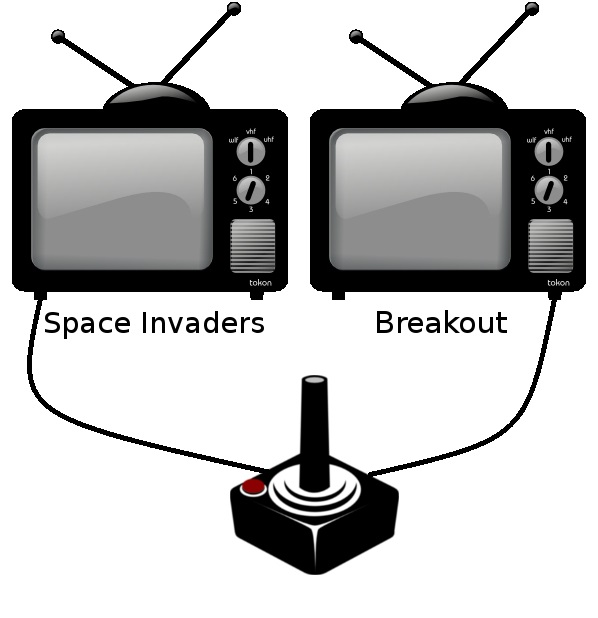
\includegraphics[width=\linewidth]{overview.jpg}
  \caption{Space Invaders and Breakout played at once with identical inputs. The images of both screens are the inputs for the agent. Based on the inputs the agent takes an action, the input for both games, to increase the scores. The agent has to balance the benefits and drawbacks of its actions for both games.  }
  \label{fig:overview}
\end{figure}
    
\subsection{Related Works}
We were inspired by the paper "Human-level control through deep reinforcement learning" \cite{Mnih2015}, which proposed an approach how to train convonlutional neural networks on classic Atari 2600 games. In the mentioned paper the authors were able to train an agent with skills classified higher than a professional human games tester. In the beginning we try to reproduce the results of this paper. After successfully implementing this architecture we combine two games together.

    	 
%        \begin{itemize}
%            \item Related and previous work on your topic
%            \item A small overview of the SOTA (state-of-the-art)
%            \item What is new/different in your approach?
%            \item $\dots$
%        \end{itemize}

\section{Dataset}
For our project we decided to use OpenAI Gym as framework for the game. OpenAI Gym is a toolkit for developing and comparing reinforcement learning algorithms implemented in Python. It allows us to gain information about the current state of the game in form of rewards and images. Instead of images it is also possible to use the memory of the current state of the game to directly access the positions of all entities in the game. It has also an API to control the agent in the selected environment.
	
Due to the fact that we use an reinforcement learning approach for our project, we do not need any labeled data and use the OpenAI Gym framework to gather inputs for our neural network. The input for the network is either current memory (states / positions / scores) of the game or images. The output on the other hand is an amount of actions taken (left / right / shoot). As score function we will use the rewards, that we can access from the Open AI Gym API.

%    \begin{itemize}
%        \item Are you working with an existing dataset or is data collection part of your project?
%        \item Explain the general nature of your data (show examples if beneficial) and provide information how you collected your dataset
%        \item Does your data provide the labels necessary for training?
%        \item Explain possible problems with the dataset
%        \item What are your inputs and outputs?
%        \item $\dots$
%    \end{itemize}

\section{Methodology}
\subsection{Architecture}
As already mentioned in the introduction we try to implement the already existing architecture of a \gls{dqn}. After the performance evaluation of a \gls{dqn}, we try to optimize this architecture to improve the results by adding BatchNorm or MaxPool layers, since the original approach did only use Conv, ReLU and FC layers. Then two things could be done for playing two games at once; Either we train one network on both games simultaneously or we try to train two different networks, each for one of the games and then have another way of selecting which input-action to take. This could be done by either taking the average or the argmax of the outputs of the networks.
%One other thing we could consider to enhance the performance of our neural network is the usage of Capsule layers \cite{Hinton2017}.

As framework for our implementation we use PyTorch.

\subsection{Training}
At first we do not use pretrained networks, but train the network from scratch. During the training we might want to use a population based approach \cite{Jaderberg2017} for hyperparameter optimization. With population based training we try to accelerate the training and also gain performance benefits. For comparisions between different architectures we use cross validation.

If training takes too much time we could use pretrained networks for the combination of the two games and just train the network combining both outputs.

\subsection{Ressource management}
In our project we want to use the Google Cloud Platform and also the machines of the lab for a faster training on GPUs. For development and document sharing we considered to use GitHub.



%
%    Describe all the different phases/components/steps on how you are planning to solve your previously stated problem. Try to give us a clear picture of your methodology and remember that the project's focus is on deep learning. Try to elaborate on the following points:
%    \begin{itemize}
%        \item Network architecture(s)
%        \item Transfer learning and training from scratch
%        \item Resource management (please consider GPU memory)
%        \item $\dots$
%    \end{itemize}

\subsection{Division of labour}
The implementation of our project is subdivided in the tasks integration of OpenAI, network architecture, training / optimization methods and evaluation / visualization of the outcomes. 

We record our progress continuously and work on the drafts for the poster and the paper in teams of two. The final work on the poster and the paper we will do with the entire team.

\section{Outcome}
We try to build an agent which is capable of playing Breakout and Space Invaders at once with one shared input and achieves a decent score. We evaluate our own network performance and compare it with the single game results from the paper and other existing implementations, which are also provided by OpenAI Gym. The resulting network will probably perform worse than current state-of-the-art networks, since it depends on two games at the same time.
    
{\small
\bibliographystyle{ieee}
\bibliography{bib}
}

\end{document}